\chapter{Zustandsgleichung, Strahlung und Vakuumenergie}

\lectureoverview{Die Geschichte eines homogenen Universums ist weitgehend die Geschichte seines Skalenfaktors \(a(t)\). Die Friedmann-Gleichung gibt die Geometrie vor, doch die Zustandsgleichung der Materie bestimmt, wie sich die Energiedichte bei der Expansion des Raums verändert. Zunächst leiten wir \(\rho\propto a^{-3(1+w)}\) aus der Arbeit eines Fluids her, bestimmen dann \(P=\rho/3\) für Strahlung durch die Übertragung des Photonimpulses und identifizieren schließlich die Vakuumenergie anhand von \(P=-\rho\). Positive Vakuumenergie führt zu einer de-Sitter-Expansion; Krümmung und Vorzeichen der kosmologischen Konstante führen zu Lösungen mit einem Übergang von Kontraktion zu Expansion (Bounce) beziehungsweise mit erneutem Kollaps, die sich als einfache mechanische Systeme deuten lassen.}

\section{Der Skalenfaktor und das fehlende Stoffgesetz}

Rufen wir uns zunächst in Erinnerung, worum es geht. In der Näherung eines homogenen und isotropen Universums ist die kosmologische Entwicklung im Wesentlichen durch eine Funktion bestimmt: \(a(t)\). Diese Funktion zu kennen beantwortet zwar nicht jede Frage über das Universum, doch sie legt Entfernungen, Expansionsraten und die Abfolge der großräumigen Entwicklungsphasen fest. In dieser Vorlesung geht es noch nicht darum, diese Phasen durch Beobachtungen nachzuweisen. Vielmehr leiten wir aus grundlegender Physik die Zustandsgleichungen her, die solche Modelle ermöglichen.

Zwei Referenzmodelle sind uns bereits begegnet:
\begin{equation}
a(t)\propto t^{2/3}
\qquad\text{(matter domination)},
\end{equation}
und
\begin{equation}
a(t)\propto t^{1/2}
\qquad\text{(radiation domination)}.
\end{equation}
Keines dieser Gesetze gilt zu allen Zeiten exakt. Strahlung liefert eine nützliche Näherung für frühe Zeiten, Materie eine für die spätere Zwischenphase; Vakuumenergie verändert schließlich erneut das Verhalten zu späten Zeiten. Die unmittelbare Frage ist nicht, wie Beobachtungen diese Phasen sichtbar machen, sondern wodurch sich die entsprechenden rechten Seiten der Friedmann-Gleichung unterscheiden.

\begin{figure}[htbp]
\centering
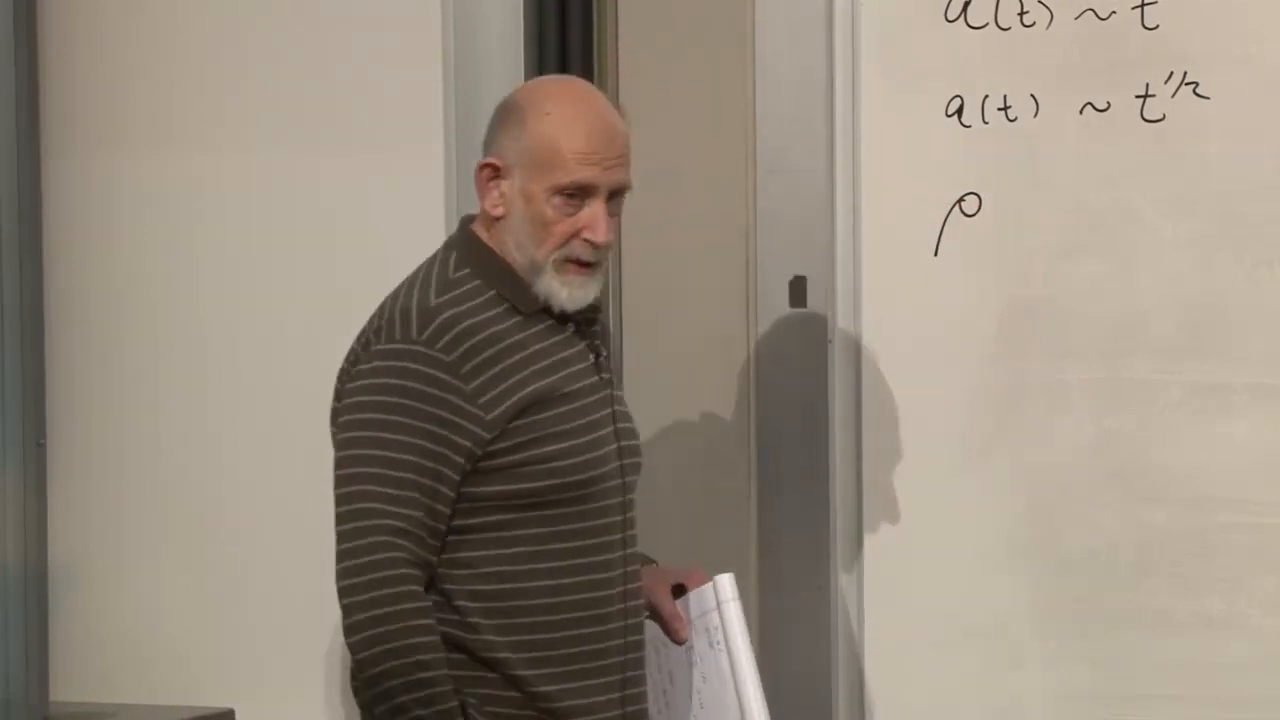
\includegraphics[width=0.72\textwidth]{lecture_05_figure_02.png}
\caption{Die wiederholten Potenzgesetze für den Skalenfaktor und das neu eingeführte Dichtesymbol. Dies ist ein Übergangszustand an der Tafel, keine abgeschlossene Herleitung.}
\label{fig:c05-review-board}
\lectureframe{00:03:18.380}
\end{figure}

Die fehlende Verbindung ist die Zustandsgleichung. Sie bestimmt, wie sich die Energiedichte auf der rechten Seite der Friedmann-Gleichung mit dem Skalenfaktor verändert. Die beiden Referenzgesetze lauten
\begin{equation}
\rho_{\text{matter}}=\frac{\rho_0}{a^3},
\qquad
\rho_{\text{rad}}=\frac{\rho_0}{a^4}.
\label{eq:c05-benchmark-densities}
\end{equation}
Materie wird durch die Volumenzunahme verdünnt, und das Volumen wächst wie \(a^3\). Die Strahlungsdichte fällt um eine zusätzliche Potenz von \(a\). Wir wollen beide Gesetze als Konsequenzen des Zusammenhangs zwischen Druck und Energiedichte verstehen.

\section{Vom Druck zum Skalierungsgesetz für die Dichte}

Eine Zustandsgleichung kann allgemein Dichte, Druck, Temperatur und weitere Größen umfassen. Für die hier betrachteten kosmologischen Komponenten verwenden wir die praktische Form mit konstantem \(w\):
\begin{equation}
P=w\rho,
\label{eq:c05-eos}
\end{equation}
Dabei charakterisiert \(w\) das Fluid. An der Tafel steht ein großes \(W\); wir verwenden das übliche kleine \(w\). Diese lineare Form umfasst die wichtigen Fälle, die wir im Folgenden betrachten. Sie ist jedoch eine vereinfachende Annahme und kein Gesetz, dem jedes denkbare Fluid gehorcht.

Bei nichtrelativistischer Materie wird die Energiedichte von der Ruheenergie dominiert. Bezeichnen \(n\) die Teilchendichte und \(m\) die Teilchenmasse, gilt schematisch
\begin{equation}
\rho\simeq nmc^2.
\end{equation}
Der Faktor \(c^2\) macht selbst eine geringe Ruhemasse zu einem enormen Energiespeicher; die vollständige Annihilation eines Staubkorns würde eine makroskopische Energiemenge freisetzen. Druck entsteht dagegen durch Impulsübertragung, wenn Teilchen gegen eine Wand stoßen, und ist von der Größenordnung \(nmv^2\). Eine Bowlingkugel überträgt mehr Impuls als ein Tischtennisball, doch in einem kalten Gas gilt für jede relevante Geschwindigkeit \(v\ll c\). Daher
\begin{equation}
\frac{P}{\rho}\sim\frac{v^2}{c^2}\ll1,
\qquad
w\simeq0.
\label{eq:c05-dust-eos}
\end{equation}
Strahlung bewegt sich mit \(c\) und erfüllt diese Näherung daher nicht. Wir werden ihren Wert von \(w\) herleiten, statt ihn vorauszusetzen.

Wir brauchen nun ein allgemeines Verfahren, das aus der Zustandsgleichung~\eqref{eq:c05-eos} ein Skalierungsgesetz für \(\rho\) macht. Dafür genügt ein Kasten im Labor. Galaxien lassen sich zwar nicht buchstäblich in einen Kasten setzen, doch nach einer Grobkörnung verhalten sie sich wie Teilchen, und der Zusammenhang zwischen Energie und Druck lässt sich lokal herleiten.

\begin{figure}[htbp]
\centering
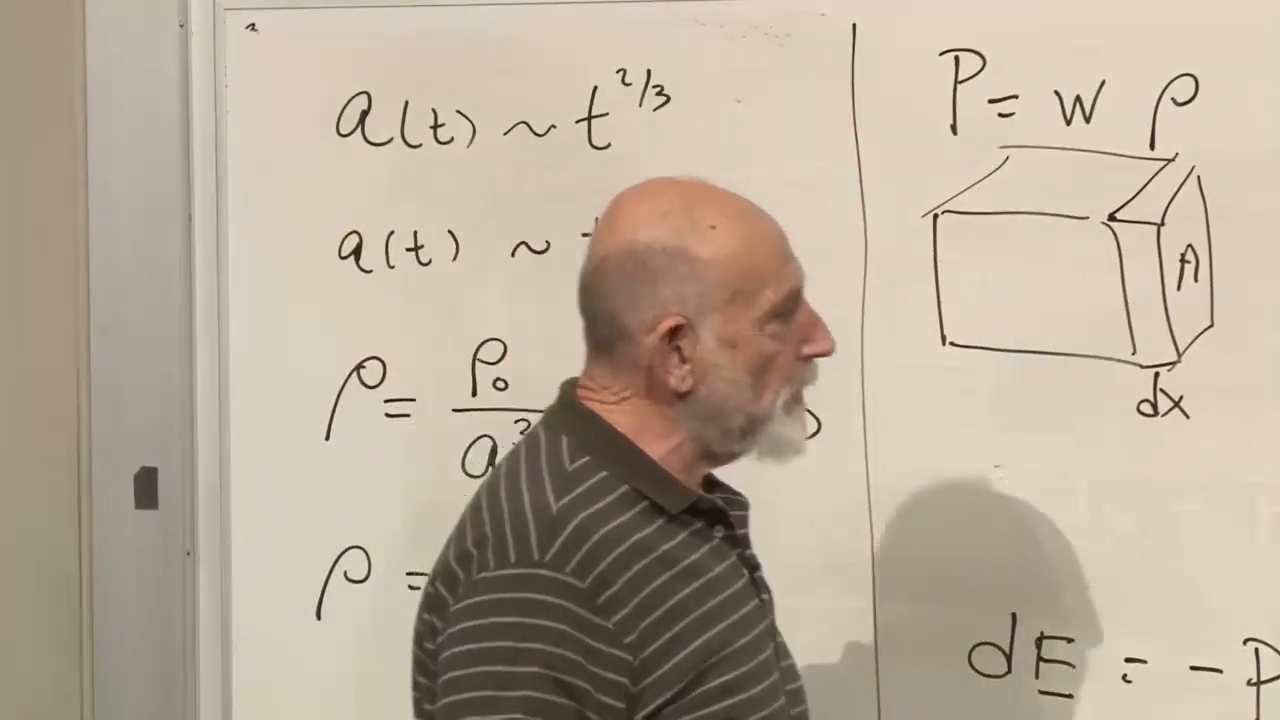
\includegraphics[width=0.86\textwidth]{lecture_05_figure_03.png}
\caption{Zustandsgleichung, wiederholte Dichteskalierungen und thermodynamischer Kasten auf einer Tafel. Der Vortragende verdeckt einen Teil der vorherigen Notizen; das Bild dient daher zur Veranschaulichung des Aufbaus und der sichtbaren Gleichungen, nicht als vollständige Abschrift.}
\label{fig:c05-box-board}
\lectureframe{00:13:39.612}
\end{figure}

Auf der linken Tafelseite stehen die wiederholten kosmologischen Skalierungen, rechts beginnt die Argumentation mit dem Kasten. Zusammengenommen verknüpfen die sichtbaren Inhalte
\begin{equation}
\rho_{\text{matter}}=\frac{\rho_0}{a^3},
\qquad
\rho_{\text{rad}}=\frac{\rho_0}{a^4},
\qquad
P=w\rho.
\end{equation}
Unsere Aufgabe ist es, die beiden Dichtegesetze aus der Zustandsgleichung herzuleiten.

Eine Wand hat die Fläche \(A\). Wir verschieben sie um \(dx\) nach außen, sodass
\begin{equation}
dV=A\,dx.
\end{equation}
Druck ist Kraft pro Fläche, also wirkt auf die Wand die Kraft \(PA\). Das Gas verrichtet die Arbeit \(PA\,dx=P\,dV\), und die im Inneren verbleibende Energie nimmt ab.
\begin{equation}
dE=-P\,dV.
\label{eq:c05-work-law}
\end{equation}
\begin{figure}[htbp]
\centering
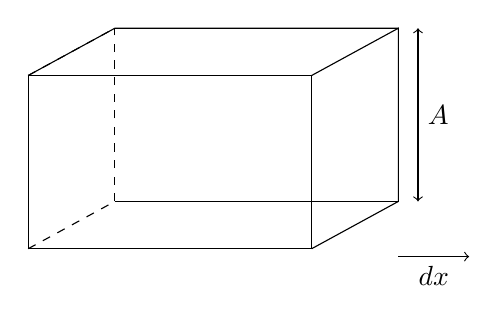
\begin{tikzpicture}[scale=1.0]
\draw (0,0) -- (3.6,0) -- (3.6,2.2) -- (0,2.2) -- cycle;
\draw (3.6,0) -- (4.7,0.6) -- (4.7,2.8) -- (3.6,2.2);
\draw (0,2.2) -- (1.1,2.8) -- (4.7,2.8);
\draw (1.1,0.6) -- (4.7,0.6);
\draw[dashed] (0,0) -- (1.1,0.6);
\draw[dashed] (0,2.2) -- (1.1,2.8);
\draw[dashed] (1.1,0.6) -- (1.1,2.8);
\draw[<->] (4.95,0.6) -- (4.95,2.8);
\node[right] at (4.95,1.7) {\(A\)};
\draw[->] (4.7,-0.1) -- (5.6,-0.1);
\node[below] at (5.15,-0.1) {\(dx\)};
\end{tikzpicture}
\caption{Eine klare Rekonstruktion des thermodynamischen Kastens mit der Wandfläche \(A\) und der Verschiebung \(dx\).}
\label{fig:c05-box-redraw}
\end{figure}

Die Gesamtenergie beträgt
\begin{equation}
E=\rho V.
\end{equation}
Differenzieren ergibt
\begin{equation}
d(\rho V)=\rho\,dV+V\,d\rho.
\end{equation}
Einsetzen in Gleichung~\eqref{eq:c05-work-law} ergibt
\begin{equation}
\rho\,dV+V\,d\rho=-P\,dV.
\end{equation}
Setzen wir \(P=w\rho\) ein:
\begin{equation}
V\,d\rho=-(1+w)\rho\,dV.
\end{equation}
Das Ergebnis führt auf die gesuchte Gleichung hin, ist aber noch nicht ganz dort. Wir dividieren durch \(\rho V\).
\begin{equation}
\frac{d\rho}{\rho}=-(1+w)\frac{dV}{V}.
\end{equation}
\begin{figure}[htbp]
\centering
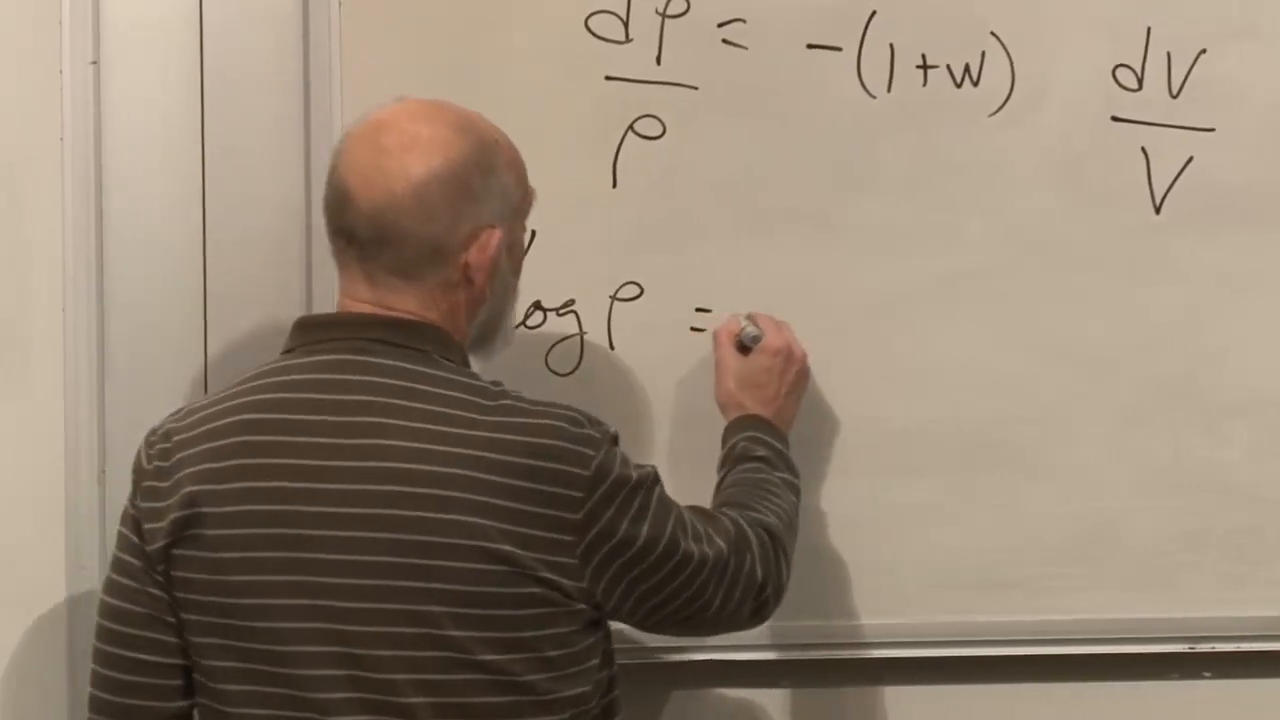
\includegraphics[width=0.78\textwidth]{lecture_05_figure_04.png}
\caption{Die separierte Gleichung für Dichte und Volumen sowie der Beginn der logarithmischen Integration. Die vollständige rechte Seite ist aus der vorherigen Algebra rekonstruiert, nicht aus verdeckten Bildpunkten.}
\label{fig:c05-log-board}
\lectureframe{00:15:35.600}
\end{figure}

Das Bild zeigt die separierte Gleichung und den Beginn von \(\log\rho=\). Führen wir die Integration direkt zu Ende:
\begin{equation}
d(\log\rho)=-(1+w)\,d(\log V),
\end{equation}
also
\begin{equation}
\log\rho=-(1+w)\log V+\text{const.}
\end{equation}
Nach dem Exponenzieren erhalten wir
\begin{equation}
\rho\propto V^{-(1+w)}.
\end{equation}
Dies ist das Dichte-Volumen-Gesetz.

Kehren wir nun vom Kasten zur Kosmologie zurück. Nur eine Wand zu verschieben war eine bequeme Herleitung, keine Annahme anisotroper Expansion. Werden alle drei Richtungen gleichmäßig ausgedehnt, ergibt sich dieselbe Arbeitsbeziehung, und ein mitbewegtes Volumen skaliert wie
\begin{equation}
V\propto a^3.
\end{equation}
Folglich
\begin{equation}
\boxed{\rho\propto a^{-3(1+w)}}.
\label{eq:c05-density-scaling}
\end{equation}
In \(d\) räumlichen Dimensionen würde der Exponent \(3\) durch \(d\) ersetzt; der Rest der Herleitung bleibt unverändert.

\section{Erste Anwendungen: Materie und Strahlung}

Nun können wir die bekannten Formeln als Konsequenzen herleiten, statt sie vorauszusetzen.

Für nichtrelativistische Materie setzen wir
\begin{equation}
w=0.
\end{equation}
Dann gilt
\begin{equation}
\rho\propto a^{-3},
\end{equation}
und damit genau das Verdünnungsgesetz für Materie.

Für Strahlung setzen wir vorläufig
\begin{equation}
w=\frac13.
\end{equation}
Wenn dies zutrifft, dann
\begin{equation}
\rho\propto a^{-3(1+1/3)}=a^{-4}.
\end{equation}
Die zusätzliche inverse Potenz entspricht also \(w=1/3\). Offen bleibt, diesen Wert aus der Physik der Photonen herzuleiten.

\section{Warum der Strahlungsdruck ein Drittel der Energiedichte beträgt}

Strahlung lässt sich als elektromagnetische Welle oder als masseloses Teilchen beschreiben. Wir betrachten Photonen und berechnen den Druck eines Photonengases in einem Kasten. Der Kasten ist zweidimensional gezeichnet, doch das Gas und seine Winkelverteilung sind dreidimensional. Die Photonen bewegen sich mit Lichtgeschwindigkeit und werden an den vorläufigen Wänden elastisch reflektiert.

Nehmen wir zunächst an, alle Photonen hätten dieselbe Energie \(\epsilon\). Diese Vereinfachung entfällt, sobald wir die Beiträge unterschiedlicher Energien addieren. Bezeichne \(\vec{\pi}\) den Impulsvektor eines Photons; die übliche Bezeichnung \(p\) vermeiden wir, weil \(P\) bereits für den Druck steht. Für ein masseloses Teilchen gelten die folgenden Beziehungen.
\begin{equation}
\epsilon=c\,\pi,
\end{equation}
mit \(\pi=|\vec{\pi}|\). In den hier verwendeten Einheiten gilt \(c=1\), also
\begin{equation}
\epsilon=\pi.
\end{equation}
Ist \(\nu\) die Photonenzahldichte, so ist die Energiedichte
\begin{equation}
\rho=\epsilon\,\nu.
\end{equation}
Die \(x\)-Achse stehe senkrecht auf einer Wand. Während eines kurzen Zeitintervalls \(\Delta t\) erreicht ein Photon, das sich unter dem Winkel \(\theta\) zu dieser Normalen bewegt, die Wand nur dann, wenn es innerhalb einer Schicht der Dicke
\begin{equation}
\Delta x=\Delta t\cos\theta.
\end{equation}
startet. Bei der Reflexion wechselt die \(x\)-Komponente seines Impulses das Vorzeichen. Der auf die Wand übertragene Impuls ist daher
\begin{equation}
\Delta \pi_x=2\epsilon\cos\theta.
\end{equation}
Kraft ist die Impulsübertragung pro Zeiteinheit, ein einzelner Stoß trägt also \(\Delta \pi_x/\Delta t\) bei. Die Schicht enthält \(\nu A\Delta x\) Photonen, doch nur die Hälfte davon bewegt sich auf die Wand zu. Relevant ist somit die Anzahl \(\tfrac12 \nu A\Delta x\). Teilen wir die Gesamtkraft durch die Wandfläche \(A\), erhalten wir
\begin{align}
P(\theta)
&=
\frac{1}{A}
\left(\frac{2\epsilon\cos\theta}{\Delta t}\right)
\left(\frac12 \nu A\Delta x\right) \\
&=
\epsilon\nu\cos\theta\frac{\Delta x}{\Delta t} \\
&=
\epsilon\nu\cos^2\theta \\
&=
\rho\cos^2\theta.
\end{align}
Das Ergebnis hängt vom Winkel ab, da es nur den Beitrag der Photonen erfasst, die sich in eine Richtung bewegen.

\begin{figure}[htbp]
\centering
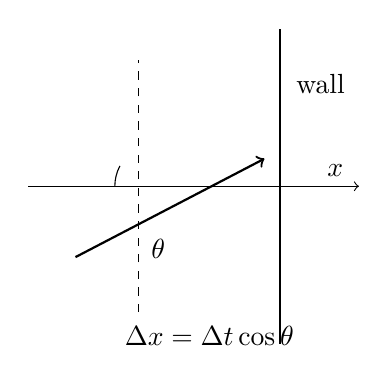
\begin{tikzpicture}[scale=1.0]
\draw[thick] (0,0) -- (0,4);
\draw[->] (-3.2,2) -- (1.0,2);
\node[above] at (0.7,2) {\(x\)};
\draw[dashed] (-1.8,0.4) -- (-1.8,3.6);
\node[below] at (-0.9,0.35) {\(\Delta x=\Delta t\cos\theta\)};
\draw[->,thick] (-2.6,1.1) -- (-0.2,2.35);
\node[below] at (-1.55,1.45) {\(\theta\)};
\draw (-2.1,2) arc[start angle=180,end angle=152,radius=0.55];
\node[right] at (0.08,3.3) {wall};
\end{tikzpicture}
\caption{Photonimpuls, der unter dem Winkel \(\theta\) auf eine Wand trifft: die Geometrie zur Herleitung des Strahlungsdrucks.}
\label{fig:c05-photon-pressure}
\end{figure}

Wir mitteln über die isotrope Verteilung. Sei \(\mathbf n=(n_x,n_y,n_z)\) der Einheitsvektor in Richtung eines Photons. Dann gilt
\begin{equation}
n_x=\cos\theta,
\qquad
n_x^2+n_y^2+n_z^2=1.
\end{equation}
In einem isotropen Gas sind die Mittelwerte von \(n_x^2\), \(n_y^2\) und \(n_z^2\) gleich. Mitteln wir die obige Identität,
\begin{equation}
\langle n_x^2\rangle+\langle n_y^2\rangle+\langle n_z^2\rangle=1,
\end{equation}
so folgt wegen der Symmetrie, dass jeder Term gleich ist:
\begin{equation}
\langle n_x^2\rangle=\langle \cos^2\theta\rangle=\frac13.
\end{equation}
Daher
\begin{equation}
P=\rho\langle \cos^2\theta\rangle=\frac{\rho}{3}.
\end{equation}
Die Zustandsgleichung der Strahlung lautet somit
\begin{equation}
P=\frac13\rho,
\qquad
w=\frac13.
\end{equation}
Der Faktor \(1/3\) entspricht der Anzahl räumlicher Richtungen, auf die sich der quadrierte Einheitsvektor verteilt. In \(d\) isotropen räumlichen Dimensionen ergäbe dieselbe Überlegung \(\langle n_x^2\rangle=1/d\). Damit ist die zu Beginn angekündigte mikroskopische Herleitung abgeschlossen.

\subsection{Fragen zur Herleitung des Strahlungsdrucks}

\begin{classroomqa}
\audiencequestion{Müssen alle Photonen dieselbe Energie haben?}
\lecturerresponse{Nein. Führen Sie die Rechnung für jedes Energieintervall gesondert durch. Jedes Intervall trägt einen Druck bei, der einem Drittel seiner eigenen Energiedichte entspricht. Daher bleibt beim Summieren über das Spektrum \(P=\rho/3\) erhalten. Die Annahme gleicher Energien diente nur dazu, die Schreibweise kurz zu halten. \lecturetimestamp{00:39:08--00:39:36}}
\end{classroomqa}

\begin{classroomqa}
\audiencequestion{Erhielte man mit absorbierenden schwarzen Wänden dasselbe Ergebnis wie mit perfekten Spiegeln, und wo befindet sich die Wand im leeren Raum?}
\lecturerresponse{Eine schwarze Wand im thermischen Gleichgewicht absorbiert und emittiert Strahlung erneut, wodurch dieselbe mittlere Impulsbilanz entsteht. Der kosmologische Raum hat keine tatsächliche Wand; die Oberfläche ist eine gedachte Grenze. Für jedes Photon, das nach außen tritt, sorgt die Isotropie im Mittel für einen entsprechenden einwärts gerichteten Fluss, sodass sich an der lokalen Rechnung des Impulsstroms nichts ändert. Bei der Strahlung im Lehrsaal handelt es sich hauptsächlich um die thermische kosmische Mikrowellenhintergrundstrahlung, für die dieses Gleichgewichtsbild besonders naheliegt. \lecturetimestamp{00:39:37--00:41:19}}
\end{classroomqa}

\begin{classroomqa}
\audiencequestion{Verändert die Quantenstatistik \(P=\rho/3\)?}
\lecturerresponse{Nein. Die Bose-Statistik bestimmt, wie Photonen die verfügbaren Moden besetzen, und damit das Spektrum und die gesamte Größe \(\rho\). Der isotrope Spannungstensor masseloser Teilchen bleibt jedoch gleich einem Drittel dieser Energiedichte. \lecturetimestamp{00:41:51--00:42:02}}
\end{classroomqa}

\begin{classroomqa}
\audiencequestion{Was geschieht, wenn Photonen miteinander streuen?}
\lecturerresponse{Die gewöhnliche Photon-Photon-Streuung ist extrem schwach; ihr Beitrag ist hier daher vernachlässigbar. Bei hinreichend hoher Temperatur und Dichte können Stöße Elektron-Positron-Paare erzeugen und den effektiven Teilcheninhalt sowie die Zustandsgleichung verändern. Das ist ein realer Effekt, gehört jedoch zu einem viel heißeren Bereich als dem, der dieser Herleitung zugrunde liegt. \lecturetimestamp{00:42:02--00:43:08}}
\end{classroomqa}

\begin{classroomqa}
\audiencequestion{Was ist mit der Wandfläche \(A\) geschehen?}
\lecturerresponse{Das Zwischenergebnis ist die Kraft eines einzelnen Photons multipliziert mit der Anzahl der Photonen, die auf die Wand treffen; diese Anzahl ist proportional zu \(A\). Der Druck ist die Kraft geteilt durch die Fläche, sodass die abschließende Division \(A\) kürzt. Der Fehler an der Tafel bestand darin, den Zwischenausdruck voreilig als Druck zu bezeichnen. Fügt man den Schritt von der Kraft zum Druck wieder ein, ist die Herleitung korrigiert. \lecturetimestamp{00:43:11--00:44:01}}
\end{classroomqa}

\section{Negativer Druck und die Bedeutung von Spannung}

Bisher sind Teilchen gegen die Wände gestoßen und haben sie nach außen gedrückt. Dieses Bild führt ganz natürlich zu positivem Druck, schöpft die Möglichkeiten aber nicht aus.

\begin{classroomqa}
\audiencequestion{Kann die Energiedichte selbst negativ sein?}
\lecturerresponse{Die Quantentheorie lässt unter eingeschränkten Bedingungen negative Energiedichten zu, und eine kosmologische Konstante kann formal beide Vorzeichen haben. Solche Fälle erfordern besondere Sorgfalt und sind kein naheliegender Ausgangspunkt. Vertrauter ist der Zugang über negativen \emph{Druck}, der auch bei positiver Energiedichte auftreten kann. \lecturetimestamp{00:44:25--00:44:59}}
\end{classroomqa}

\begin{classroomqa}
\audiencequestion{Wie kann Druck negativ sein?}
\lecturerresponse{In einer eindimensionalen Welt ist ein Kasten ein Liniensegment. Frei bewegliche Teilchen stoßen an seine Enden und drücken sie nach außen; der Druck ist positiv. Verbindet man die Enden stattdessen durch eine gespannte Schnur oder Feder, zieht diese beim Auseinanderziehen der Enden nach innen. Diese nach innen gerichtete Kraft ist die Spannung und das eindimensionale Modell für negativen Druck. \lecturetimestamp{00:45:04--00:46:31}}
\end{classroomqa}

\begin{figure}[htbp]
\centering
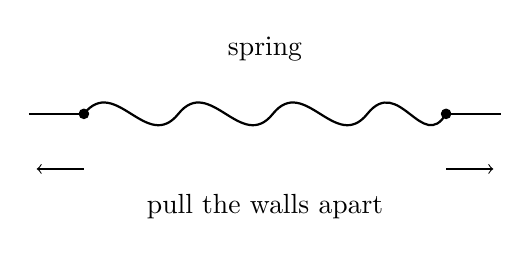
\begin{tikzpicture}[scale=1.0]
\draw[thick] (-3,0) -- (-2.3,0);
\draw[thick] (2.3,0) -- (3,0);
\draw[fill] (-2.3,0) circle (0.06);
\draw[fill] (2.3,0) circle (0.06);
\draw[thick] (-2.3,0)
.. controls (-1.9,0.5) and (-1.5,-0.5) .. (-1.1,0)
.. controls (-0.7,0.5) and (-0.3,-0.5) .. (0.1,0)
.. controls (0.5,0.5) and (0.9,-0.5) .. (1.3,0)
.. controls (1.7,0.5) and (2.0,-0.5) .. (2.3,0);
\draw[->] (-2.3,-0.7) -- (-2.9,-0.7);
\draw[->] (2.3,-0.7) -- (2.9,-0.7);
\node[below] at (0,-0.9) {pull the walls apart};
\node[above] at (0,0.55) {spring};
\end{tikzpicture}
\caption{Eine eindimensionale Feder als Analogie für negativen Druck.}
\label{fig:c05-tension}
\end{figure}

Die Arbeitsbilanz kehrt sich entsprechend um. Bei der Expansion verrichtet ein Gas mit positivem Druck Arbeit und verliert innere Energie. Zieht man die Enden gegen die Spannung nach außen, wird Energie in der Feder gespeichert. Allgemeiner können anziehende Bestandteile einander und die Begrenzung nach innen ziehen. Ein System kann daher \(\rho>0\) und \(P<0\) haben, sodass \(w<0\) gilt, ohne dass ein Widerspruch entsteht. Diese Möglichkeit ist zentral, denn Vakuumenergie weist genau diese Vorzeichen auf.

\section{Vakuumenergie und kosmologische Konstante}

Vakuumenergie wird dem leeren Raum selbst zugeschrieben. Die Quantenfeldtheorie motiviert sie durch die Nullpunktsbewegung der harmonischen Oszillatoren, die den Feldmoden entsprechen. Für die makroskopische Beschreibung müssen wir dieses mikroskopische Problem jedoch nicht lösen. Entscheidend ist, dass leerer Raum dieselbe Energiedichte hat, unabhängig davon, wo und wie groß der betrachtete Bereich ist.
\begin{equation}
\rho=\rho_0=\text{const.}
\label{eq:c05-vacuum-density}
\end{equation}
Enthält ein Bereich mit Volumen \(V\) ausschließlich Vakuumenergie, so beträgt seine Gesamtenergie
\begin{equation}
E=\rho_0 V.
\end{equation}
\begin{classroomqa}
\audiencequestion{Verändert ein Kasten die Vakuumdichte, weil er die möglichen Feldmoden einschränkt?}
\lecturerresponse{Die Gesamtenergie in einem endlichen Bereich ist geringer als die Energie im gesamten Raum, weil der Bereich ein kleineres Volumen hat; die lokale Dichte \(\rho_0\) bleibt unverändert. Reale Begrenzungen können die Modenenergien verändern und den Casimir-Effekt hervorrufen. Dieser Beitrag ist jedoch relevant, wenn die Abstände mit den betreffenden Wellenlängen vergleichbar sind. Er ist nicht die großräumige Vakuumdichte, um die es in der Kosmologie geht. \lecturetimestamp{00:50:06--00:51:25}}
\end{classroomqa}

Führen wir ein:
\begin{equation}
\Lambda=\frac{8\pi G}{3}\rho_0.
\label{eq:c05-lambda-definition}
\end{equation}
Diese Definition fasst die Kombination zusammen, die in der Friedmann-Gleichung auftritt. Die umgekehrte Beziehung lautet
\begin{equation}
\rho_0=\frac{3\Lambda}{8\pi G}.
\end{equation}
Der Parameter \(\Lambda\) ist die kosmologische Konstante. Eine positive, annähernd konstante Komponente, die die späte beschleunigte Expansion antreibt, wird gemeinhin als dunkle Energie bezeichnet.

Die Abhängigkeit vom Skalenfaktor steht bereits fest. Kehren wir daher die Argumentation mit dem Kasten um, um den Druck zu bestimmen. Da \(d\rho_0=0\) gilt,
\begin{equation}
dE=d(\rho_0V)=\rho_0\,dV.
\end{equation}
Andererseits gilt weiterhin die thermodynamische Arbeitsbeziehung
\begin{equation}
dE=-P\,dV.
\end{equation}
Schreiben wir \(P=w\rho_0\), dann
\begin{equation}
dE=-w\rho_0\,dV.
\end{equation}
Der Vergleich ergibt
\begin{equation}
w=-1.
\end{equation}
und somit
\begin{equation}
P=-\rho.
\end{equation}
Die Analogie mit der Feder bereitete auf dieses Vorzeichen vor. Positive Vakuumenergie hat negativen Druck, negative Vakuumenergie positiven Druck. Astronomische Messungen von \(w\) untersuchen, ob sich die Komponente zu späten Zeiten tatsächlich wie ein sich nicht verdünnendes Vakuum verhält: Je näher \(w\) an \(-1\) liegt, desto ähnlicher ist das Verhalten dem in Gleichung~\eqref{eq:c05-vacuum-density} beschriebenen.

\begin{classroomqa}
\audiencequestion{Ist \(P=-\rho\) die Zustandsgleichung eines leeren Universums, und lässt sich \(\rho_0\) berechnen?}
\lecturerresponse{Es ist die Zustandsgleichung des leeren Raums, wenn Vakuumenergie vorhanden ist. Ihr Betrag ist viel schwieriger zu bestimmen. Jedes Quantenfeld und jede Energieskala kann einen Beitrag liefern, auch Felder, die noch nicht entdeckt wurden. Daher gibt es keine anerkannte Berechnung, die den beobachteten Wert erklärt. Das Hauptproblem ist nicht, \(w=-1\) anzuschreiben, sondern zu erklären, warum die resultierende \(\rho_0\) außerordentlich klein ist. \lecturetimestamp{00:57:27--00:58:29}}
\end{classroomqa}

\section{Vakuumenergie in der Friedmann-Dynamik}

Isolieren wir die Vakuumenergie, wie wir zuvor reine Materie und reine Strahlung isoliert haben. Mit \(\rho=\rho_0\) wird die Friedmann-Gleichung zu
\begin{equation}
\left(\frac{\dot a}{a}\right)^2=\Lambda-\frac{k}{a^2},
\label{eq:c05-vacuum-friedmann}
\end{equation}
Dabei gilt \(k=+1,0,-1\) für sphärischen, flachen und hyperbolischen Raum. Zusammen mit den drei Möglichkeiten für \(k\) ergeben positives und negatives \(\Lambda\) sechs Vorzeichenfälle, auch wenn nicht jeder Fall eine reelle Lösung zulässt.

\begin{remark}
In der Vorlesung wird \(\Lambda=(8\pi G/3)\rho_0\) definiert; daher hat \(\Lambda\) hier die Dimension \(H^2\). In der verbreiteten Konvention \(G_{\mu\nu}+\Lambda_{\mathrm E}g_{\mu\nu}=8\pi G T_{\mu\nu}\) lautet der entsprechende Parameter \(\Lambda_{\mathrm E}=3\Lambda\).
\end{remark}

\subsection{Flache de-Sitter-Expansion}

Setzen wir \(k=0\). Dann gilt
\begin{equation}
\left(\frac{\dot a}{a}\right)^2=\Lambda.
\end{equation}
Für \(\Lambda>0\) wählen wir den expandierenden Zweig:
\begin{equation}
\dot a=\sqrt{\Lambda}\,a,
\end{equation}
und damit
\begin{equation}
a(t)=C\,e^{\sqrt{\Lambda}\,t}.
\end{equation}
Der Hubble-Parameter ist dann konstant:
\begin{equation}
H=\frac{\dot a}{a}=\sqrt{\Lambda}.
\end{equation}
Dies ist der de-Sitter-Raum in flacher Scheinung, benannt nach Willem de Sitter, der kurz nachdem Einstein den Begriff eingeführt hatte, im Jahr 1917 die Lösung mit kosmologischer Konstante fand. Falls \(\Lambda<0\) und zugleich \(k=0\) gilt, hat Gleichung~\eqref{eq:c05-vacuum-friedmann} keine reelle Lösung, denn \(H^2\) kann nicht negativ sein.

\begin{classroomqa}
\audiencequestion{Ist der Hubble-Parameter hier tatsächlich konstant, und hat diese Raumzeit einen Urknall?}
\lecturerresponse{Für die reine Lösung in flacher Scheinung ist \(H=\sqrt{\Lambda}\) exakt konstant. Obwohl \(a(t)\to0\) nur für \(t\to-\infty\) gilt, ist dieser Koordinatenbereich nicht geodätisch vollständig: Einige vergangenheitsgerichtete Bahnen erreichen seine Grenze in endlicher Eigenzeit. Die Formel allein beantwortet daher nicht die globale Frage nach einem Urknall. Die vollständige de-Sitter-Geometrie umfasst mehr als diesen flachen Bereich; darauf kommen wir zurück, wenn wir die Geometrie im Detail untersuchen. \lecturetimestamp{01:06:54--01:08:07}}
\end{classroomqa}

Eine schematische Friedmann-Gleichung für ein Universum mit Materie, Strahlung, Krümmung und Vakuumenergie lautet
\begin{equation}
\left(\frac{\dot a}{a}\right)^2
=
\Lambda+\frac{C_m}{a^3}+\frac{C_r}{a^4}-\frac{k}{a^2}.
\label{eq:c05-mixed-friedmann}
\end{equation}
Zu frühen Zeiten, wenn \(a\) klein ist, dominieren die inversen Potenzen und die Vakuumenergie ist vernachlässigbar. Zu späten Zeiten, wenn \(a\) groß ist, dominiert der konstante Term \(\Lambda\). Das Universum durchläuft also einen Übergang: Anfangs wird seine Entwicklung von Materie oder Strahlung bestimmt, später nähert es sich einem de-Sitter-artigen Verhalten.

Für eine Exponentialfunktion gilt \(\ddot a>0\), die Vakuumdominanz bedeutet also beschleunigte Expansion. Während des Übergangs muss die Beschleunigung nicht exakt exponentiell sein, denn Materie trägt weiterhin zu Gleichung~\eqref{eq:c05-mixed-friedmann} bei. Den Beobachtungen aus der Zeit der Vorlesung zufolge befand sich das Universum damals noch in dieser Konkurrenzphase und nicht bereits in einem reinen de-Sitter-Zustand.

\section{Fragen zur Vakuumenergie}

\begin{classroomqa}
\audiencequestion{Wenn Vakuumenergie die Energie des Grundzustands ist, wie kann sie dann negativ sein?}
\lecturerresponse{Ein bosonischer Oszillatormodus trägt \(+\tfrac12\hbar\omega\) bei, ein fermionischer Modus dagegen einen Beitrag mit umgekehrtem Vorzeichen. Die Vakuumenergie ist eine Summe über viele Felder und Skalen; bevor die Gesamtsumme bekannt ist, sind daher beide Vorzeichen möglich. Dass es Beiträge gibt, ist naheliegend. Schwierig ist zu erklären, warum ihre verbleibende Summe außerordentlich klein ist. \lecturetimestamp{01:12:00--01:14:12}}
\end{classroomqa}

\begin{classroomqa}
\audiencequestion{Führt konstantes \(w=-1\) künftig zu einem Big Rip?}
\lecturerresponse{Nein. Eine kosmologische Konstante mit \(w=-1\) führt zu einer de-Sitter-artigen exponentiellen Expansion, aber nicht zu der in endlicher Zeit auftretenden Divergenz, die als Big Rip bezeichnet wird. Dieses Szenario setzt eine hypothetische Phantomkomponente mit \(w<-1\) voraus, deren Dichte mit der Expansion des Universums zunimmt. Eine solche Komponente wird hier nicht angenommen. \lecturetimestamp{01:14:13--01:15:50}}
\end{classroomqa}

\begin{classroomqa}
\audiencequestion{Würde exakte Supersymmetrie die Vakuumenergie verschwinden lassen?}
\lecturerresponse{Sie kann die Nullpunktsbeiträge aufheben, weil jedem bosonischen Freiheitsgrad ein fermionischer zugeordnet ist. In der Natur zeigt sich jedoch keine exakte Supersymmetrie bei niedrigen Energien: Beobachtete Bosonen und Fermionen sind keine massengleichen Partner. Eine exakte Aufhebung erklärt die Vakuumenergie in der bislang beobachteten Welt daher nicht. \lecturetimestamp{01:15:51--01:16:20}}
\end{classroomqa}

\begin{classroomqa}
\audiencequestion{Wie groß ist die Diskrepanz zwischen einer natürlichen Abschätzung der Vakuumenergie und dem beobachteten Wert?}
\lecturerresponse{Die Naturkonstanten \(c\), \(\hbar\) und \(G\) legen die Planck-Einheiten fest. Die Lichtgeschwindigkeit \(c\) begrenzt die Geschwindigkeit jedes Signals, \(\hbar\) legt die universelle Skala der quantenmechanischen Unschärfe fest, und \(G\) koppelt jede Energie an die Gravitation. Daraus lassen sich eine Planck-Masse von ungefähr \(10^{-5}\) Gramm und eine Planck-Länge von ungefähr \(10^{-33}\) Zentimetern bilden. Daraus folgt eine Planck-Energiedichte von ungefähr einer Planck-Energie pro kubischer Planck-Länge. In diesen Einheiten wird die beobachtete Vakuumdichte in der Vorlesung mit etwa \(10^{-123}\) angegeben; der genaue Exponent hängt von der Konvention ab. Das Rätsel besteht darin, warum Beiträge, die natürlicherweise auf eine viel größere Skala hindeuten, ein so winziges, von null verschiedenes Ergebnis hinterlassen. \lecturetimestamp{01:16:21--01:23:12}}
\end{classroomqa}

\begin{classroomqa}
\audiencequestion{Warum waren Physiker überrascht, eine von null verschiedene kosmologische Konstante zu entdecken, wenn Beiträge zum Vakuum erwartet werden?}
\lecturerresponse{Wiederholte Verbesserungen der Beobachtungen hatten immer wieder ein mit null verträgliches Ergebnis geliefert. Das führte zu der psychologischen Erwartung, ein unbekanntes exaktes Prinzip – vielleicht in einer künftigen Theorie der Quantengravitation – erzwinge die vollständige Aufhebung. Die spätere Entdeckung widerlegte diese Erwartung. Die Überraschung war die Folge jahrzehntelang immer strengerer Nullresultate, nicht einer Herleitung, nach der die Vakuumenergie verschwinden musste. \lecturetimestamp{01:23:14--01:26:05}}
\end{classroomqa}

\begin{classroomqa}
\audiencequestion{Können Beobachtungen feststellen, ob sich dunkle Energie mit der Zeit verändert?}
\lecturerresponse{Einen abrupten Wandel in ferner Zukunft können sie nicht ausschließen. Sie können jedoch die jüngere Expansionsgeschichte über mehrere Milliarden Jahre vergleichen. Die Messung von \(w\) oder allgemeiner von \(w(a)\) prüft, ob sich die Dichte in diesem Zeitraum verändert hat. Laut Vorlesung lag die damalige Grenze nur ungefähr bei zehn Prozent; diese Zahl ist historisch. Die bleibende Aussage ist, dass \(w=-1\) einer konstanten Dichte entspricht. \lecturetimestamp{01:26:06--01:27:16}}
\end{classroomqa}

\begin{classroomqa}
\audiencequestion{Wäre das Ergebnis in einer anderen Anzahl räumlicher Dimensionen anders?}
\lecturerresponse{Die Grundstruktur bleibt erhalten. In \(d\) isotropen räumlichen Dimensionen gilt für Strahlung \(w=1/d\), und ihre Dichte fällt wie \(a^{-(d+1)}\); Lorentz-invariante Vakuumenergie hat weiterhin \(w=-1\). Die Zahlenkoeffizienten in der Friedmann-Gleichung ändern sich mit der Dimension, doch die Unterscheidung zwischen verdünnender Materie, Strahlung und nicht verdünnendem Vakuum bleibt bestehen. \lecturetimestamp{01:27:16--01:27:57}}
\end{classroomqa}

\section{Krümmung und die mechanische Analogie}

\subsection{Positive Krümmung bei positiver Vakuumenergie}

Nehmen wir \(k=+1\) und \(\Lambda>0\) an:
\begin{equation}
\left(\frac{\dot a}{a}\right)^2=\Lambda-\frac{1}{a^2}.
\label{eq:c05-closed-vacuum}
\end{equation}
Multiplizieren wir mit \(a^2\),
\begin{equation}
\dot a^2-\Lambda a^2=-1.
\label{eq:c05-inverted-oscillator}
\end{equation}
und betrachten \(a\) als Koordinate eines fiktiven Teilchens. Dann ist \(\dot a^2\) sein kinetischer Term, \(-\Lambda a^2\) ein umgedrehtes quadratisches Potenzial und die Gesamtenergie \(-1\). Der physikalisch zulässige Zweig erfüllt \(a\geq\Lambda^{-1/2}\): Das Universum zieht sich ausgehend von großer Ausdehnung zusammen, kommt am Minimum zum Stillstand und expandiert anschließend wieder.

Die exakte Lösung lautet
\begin{equation}
a(t)=\Lambda^{-1/2}\cosh(\sqrt{\Lambda}\,t).
\label{eq:c05-closed-desitter}
\end{equation}
Dabei gilt
\begin{equation}
\cosh(\sqrt{\Lambda}\,t)
=
\frac12\left(e^{\sqrt{\Lambda}\,t}+e^{-\sqrt{\Lambda}\,t}\right),
\end{equation}
Die Funktion ist symmetrisch in der Zeit. Bei \(t=0\) ist \(a=\Lambda^{-1/2}\); in beiden Zeitrichtungen wächst der Skalenfaktor exponentiell. Die geschlossene Scheinung zeigt daher eine Kontraktion, ein reguläres Minimum und eine erneute Expansion. Global betrachtet unterscheidet sie sich deutlich von der flachen exponentiellen Scheinung; dennoch überdecken beide Koordinatensysteme Bereiche derselben de-Sitter-Geometrie.

\subsection{Negative kosmologische Konstante}

Schreiben wir \(\Lambda=-|\Lambda|\). Für \(k=+1\) ist die rechte Seite von Gleichung~\eqref{eq:c05-vacuum-friedmann} für jedes \(a\) negativ, während \(H^2\geq0\) gilt. Eine reelle FRW-Lösung dieses reinen Vakuumtyps existiert nicht.

Für \(k=-1\) gilt
\begin{equation}
\left(\frac{\dot a}{a}\right)^2=-|\Lambda|+\frac{1}{a^2}.
\end{equation}
Multiplizieren wir mit \(a^2\),
\begin{equation}
\dot a^2+|\Lambda|a^2=1.
\label{eq:c05-negative-lambda-oscillator}
\end{equation}
so erhalten wir die Energiegleichung eines harmonischen Oszillators. Da \(a\geq0\) gilt, ist eine physikalische Halbperiode gegeben durch
\begin{equation}
a(t)=\frac{1}{\sqrt{|\Lambda|}}
\sin\!\left(\sqrt{|\Lambda|}\,t\right),
\qquad
0<t<\frac{\pi}{\sqrt{|\Lambda|}}.
\end{equation}
Das offene Universum beginnt bei \(a=0\), erreicht \(a_{\max}=|\Lambda|^{-1/2}\) und endet wieder in einem Big Crunch. Eine offene räumliche Geometrie garantiert also keine ewige Expansion; eine negative kosmologische Konstante kann sie umkehren. Ein sehr großes positives \(\Lambda\) würde gebundene Strukturen auseinanderreißen, ein großes negatives dagegen einen raschen erneuten Kollaps verursachen.

\begin{figure}[htbp]
\centering
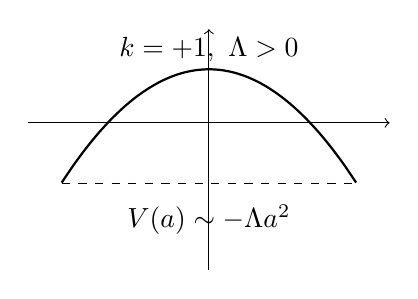
\begin{tikzpicture}[scale=0.85]
\draw[->] (-2.7,0) -- (2.7,0);
\draw[->] (0,-2.2) -- (0,1.4);
\draw[thick,domain=-2.2:2.2,smooth] plot (\x,{-0.35*(\x)^2 + 0.8});
\draw[dashed] (-2.2,-0.9) -- (2.2,-0.9);
\node at (0,-1.45) {\(V(a)\sim -\Lambda a^2\)};
\node at (0,1.1) {\(k=+1,\ \Lambda>0\)};
\end{tikzpicture}
\hspace{2em}
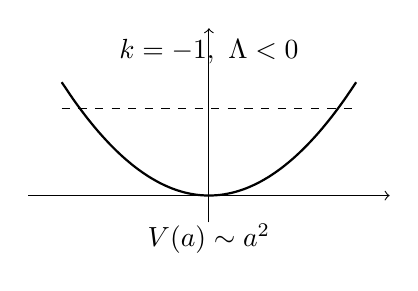
\begin{tikzpicture}[scale=0.85]
\draw[->] (-2.7,0) -- (2.7,0);
\draw[->] (0,-0.4) -- (0,2.5);
\draw[thick,domain=-2.2:2.2,smooth] plot (\x,{0.35*(\x)^2});
\draw[dashed] (-2.2,1.3) -- (2.2,1.3);
\node at (0,-0.65) {\(V(a)\sim a^2\)};
\node at (0,2.15) {\(k=-1,\ \Lambda<0\)};
\end{tikzpicture}
\caption{Schematische effektive Potenziale für den de-Sitter-Bounce bei geschlossener Geometrie und den erneuten Kollaps bei offenem Raum und negativer \(\Lambda\).}
\label{fig:c05-mechanical-potentials}
\end{figure}

\begin{classroomqa}
\audiencequestion{Sind diese Friedmann-Gleichungen wirklich Einsteins Gleichungen?}
\lecturerresponse{Ja. Es handelt sich um Einsteins Feldgleichung, nachdem die Homogenität und Isotropie die Metrik auf die einzige Funktion \(a(t)\) reduziert haben. Durch die Symmetriereduktion entfallen die meisten Tensorkomponenten; übrig bleibt diese gewöhnliche Differentialgleichung für die kosmische Expansion. \lecturetimestamp{01:43:52--01:44:05}}
\end{classroomqa}

\begin{classroomqa}
\audiencequestion{Kann der Skalenfaktor \(a\) komplex sein?}
\lecturerresponse{Nicht in den reellen klassischen FRW-Kosmologien, die hier untersucht werden. Der Skalenfaktor misst die räumliche Größe und wird als reell und nichtnegativ angenommen. Komplexifizierte Geometrien können in anderen mathematischen Ansätzen auftreten, spielen aber für die Lösungen dieser Vorlesung keine Rolle. \lecturetimestamp{01:44:06--01:44:21}}
\end{classroomqa}

\begin{classroomqa}
\audiencequestion{Gibt es einen physikalischen Grund dafür, dass der Druck eine lineare Funktion der Dichte sein muss?}
\lecturerresponse{Nein. Ein konstantes \(w\) ist praktisch und beschreibt zufällig die hier betrachteten Hauptkomponenten. Ein Gemisch aus Materie, Strahlung und Vakuum hat nicht in allen Epochen ein einziges konstantes \(w\), und für einen allgemeinen Stoff kann \(P(\rho)\) nichtlinear sein. Bei einer barotropen Flüssigkeit bestimmt \(dP/d\rho\) die quadrierte Schallgeschwindigkeit in Einheiten mit \(c=1\); ein konstantes \(w\) macht diese Ableitung konstant, aber die Natur ist dazu nicht verpflichtet. \lecturetimestamp{01:44:21--01:45:34}}
\end{classroomqa}

\section{Was Sie mitnehmen sollten}

Die Zustandsgleichung verknüpft die mikroskopische Physik mit dem zeitlichen Verlauf des Skalenfaktors. Adiabatische Arbeit in einem mitbewegten Kasten ergibt
\[
\rho\propto a^{-3(1+w)}.
\]
Für kalte Materie gilt \(w=0\) und \(\rho\propto a^{-3}\). Aus dem isotropen Impulsfluss der Photonen folgt
\[
\left\langle\cos^2\theta\right\rangle=\frac13,
\qquad
P_{\mathrm r}=\frac{\rho_{\mathrm r}}{3},
\qquad
\rho_{\mathrm r}\propto a^{-4}.
\]

Spannung macht negativen Druck physikalisch anschaulich. Für eine konstante Vakuumdichte gilt
\[
P_\Lambda=-\rho_\Lambda,
\qquad
w_\Lambda=-1.
\]
Positive Vakuumenergie führt in flacher Slicing zu einer exponentiellen de-Sitter-Expansion und in geschlossener Slicing zu einem \(\cosh\)-Bounce. Negative Vakuumenergie kann sogar ein offenes Universum zum Rekollaps bringen. In allen Vorzeichenfällen lässt sich die Friedmann-Gleichung als effektive mechanische Energiegleichung lesen. Die offene Frage ist nicht, warum Quantenfelder zur Vakuumenergie beitragen, sondern warum ihr beobachteter Nettobeitrag nahezu null, aber nicht exakt null ist.
